\label{chap:communication}
\label{sec:communication}

This chapter describes the communication interface between the GUI and the User Space, which is based on Remote Procedure Calls.

\section{Remote Procedure Calls}
\label{sec:rpc:rpc}

GUI communicates with User Space via the Google Web Toolkit RemoteService implementation.

A \emph{remote procedure call} is a method providing interaction between the client (the GUI) and the server (the Userspace). The shared class {\tt FilmTitService} \emph{defines} the FilmTitService interface, an API for the communication, by specifying the RPCs as methods with a name, a set of parameters, a return type and checked exceptions. The User Space class {\tt FilmTitBackendServer} must \emph{implement} each of the defined RPCs. The interface provides \emph{asynchronous} RPC methods -- the responses are processed by \emph{callbacks}. A class in {\tt cz.filmtit.client.callables} may \emph{invoke} the RPC, passing the required parameters to the GWT RPC mechanism which ensures their delivery to the server and the execution of the implementation method.

The callable class must implement an asynchronous callback by implementing the methods {\tt onSuccess()} and {\tt onFailure()}, which are called by the GWT RPC mechanism when the RPC \emph{returns}, i.e.\ returns a value or fails with an exception and the result is received by GUI. Failure is defined as the RPC server implementation throwing an exception, which is passed as a parameter to {\tt onFailure()}. Otherwise, the returned value is passed to {\tt onSuccess()}.
In case of common points of failure that do not qualify as an exceptional state, such as user registration attempt with an already existing username, the common failure is typically signalled by the return value instead (typically a null or a false).

The RPC is always invoked from the client, because JavaScript security policies do not allow to handle incoming calls.
Therefore, in case the User Space needs to actively contact the GUI without the GUI having sent a request before,
this has to be implemented in the GUI by polling.

Most of the RPCs can only be invoked by a logged in user. Such RPCs always have the sessionID as their first parameter to authenticate the user and can throw an {\tt InvalidSessionIdException}.
A {\tt sessionID} is a unique identifier of a logged in user, valid for 1 hour (or 1 month if the user decided to be ``permanently logged in''), managed by the User Space.

\section{Manipulating Documents}
\label{sec:rpc:doc}

TODO: See shared Document, see shared Chunk, see shared TimedChunk.
(Needed to understand e.g. movieTitle or ChunkIndex.)

A document is always identified by its {\tt documentID} (a long number generated by User Space on document creation), therefore most of the methods have the {\tt documentID} as one of their parameters.

A chunk in the document can always be identified by its {\tt ChunkIndex}, but for convenience in some cases the whole chunk is sent instead.
\todo{we should most probably send only the ChunkIndex always (except for saveSourceChunks of course)}

First, we introduce all the RPCs manipulating the documents. Then, we illustrate a typical sequence of RPCs invoked on document creation.

\subsection{Whole Document Operations}

\subsubsection{DocumentResponse createNewDocument(String sessionID, String documentTitle, String movieTitle, String language, String moviePath)}

Creates the document
(without source chunks, which have to be added by calling {\tt saveSourceChunks}).
Returns the {\tt documentID}, together with media source suggestions based on {\tt movieTitle}.
     	
\subsubsection{Void selectSource(String sessionID, long documentID, MediaSource selectedMediaSource)}
Sets the media source of the document. The media source represents the movie or series which the subtitles come from.

\subsubsection{List<Document> getListOfDocuments(String sessionID)}
Returns all documents owned by the user, ordered by date and time of last change.

\subsubsection{Document loadDocument(String sessionID, long documentID)}
Returns the document with the given documentID, with source chunks but without translation suggestions (these have to be explicitely requested by getTranslationResults).

\subsubsection{Void changeDocumentTitle(String sessionID, long documentID, String newTitle)}
Sets a different title for the document.

\subsubsection{List<MediaSource> changeMovieTitle(String sessionID, long documentID, String newMovieTitle)}
Returns media source suggestions based on {\tt newMovieTitle}.
The movie title is not changed yet:
this is only done on calling {\tt selectSource}.
     	
\subsubsection{Void deleteDocument(String sessionID, long documentID)}
Remove the given document from the list of user\'s documents.
(The data might not be discarded immediately
as the translations still might be used to enrich the translation memory)	 

\subsection{Source Subtitles Operations}

\subsubsection{Void saveSourceChunks(String sessionID, List<TimedChunk> chunks)}
Save the given source chunks as the contents of the given document
(which was already created by calling {\tt createNewDocument}).

\subsubsection{Void setChunkStartTime(String sessionID, ChunkIndex chunkIndex, long documentID, String newStartTime)}
Change the start time of the given chunk to the new value. The value must be in the SRT format, i.e. hh:mm:ss,ttt.

\subsubsection{Void setChunkEndTime(String sessionID, ChunkIndex chunkIndex, long documentID, String newEndTime)}
Change the end time of the given chunk to the new value. The value must be in the SRT format, i.e. hh:mm:ss,ttt.

\subsubsection{Void setChunkTimes(String sessionID, ChunkIndex chunkIndex, long documentID, String newStartTime, String newEndTime)}
Change the start time and end time of the given chunk to the values. The values must be in the SRT format, i.e. hh:mm:ss,ttt.

\subsubsection{TranslationResult changeText(String sessionID, TimedChunk chunk, String newDbForm)}
Change the source text of the chunk,
resulting in new translation suggestions
which are sent as the result.

\subsubsection{Void deleteChunk(String sessionID, ChunkIndex chunkIndex, long documentID)}
Remove the chunk from the document, together with its translation if it exists.

\subsection{Target Subtitles Operations}

\subsubsection{TranslationResult getTranslationResults(String sessionID, TimedChunk chunk)}
Get the list of possible translations of the given chunk.
The {\tt TranslationResult} instance contains zero or more translation suggestions, which come from the Translation Memory and/or the Machine Translation System.

\subsubsection{List<TranslationResult> getTranslationResults(String sessionID, List<TimedChunk> chunks)}
Get the list of lists of possible translations of the given chunks.
Each TranslationResult instance contains zero or more translation suggestions, which come from the Translation Memory and/or the Machine Translation System.

\subsubsection{Void stopTranslationResults(String sessionID, List<TimedChunk> chunks)}
Stop generating translation results for the given chunks
(to be called after getTranslationResults has been called
with the given chunks but the results are suddenly not needed anymore).

\subsubsection{Void setUserTranslation(String sessionID, ChunkIndex chunkIndex, long documentID, String userTranslation, long chosenTranslationPairID)}
Save the user translation of the given chunk (no matter whether it is user\'s own translation or a suggestion taken over or post-edited).
The ID of the {\tt TranslationPair} chosen for post-editing is also sent, providing feedback which then can be used to improve future suggestions.

\subsection{Document Creation}

The sequence diagram \ref{rpc:sd:document_creation} illustrates a typical sequence of RPCs invoked to create a document, including interaction with the Freebase service and the Core.

First, an empty document is created by the {\tt createNewDocument} RPC. The Freebase service is queried for suggestions on the actual movie or series matching the given {\tt movieTitle}, from which one is then selected by the {\tt selectSource} RPC -- this enables the Core to provide translation suggestions ranked according to the closeness of movie genres. Meanwhile, the {\tt saveSourceChunks} RPC is invoked to store the contents of the document once the subtitles file is parsed.

When both {\tt selectSource} and {\tt saveSourceChunks} have returned, the {\tt getTranslationResults} RPC starts to be iteratively invoked to obtain translation suggestions, generated by the Core, until the whole document gets translation suggestions.

\begin{figure}[h]
\begin{center}
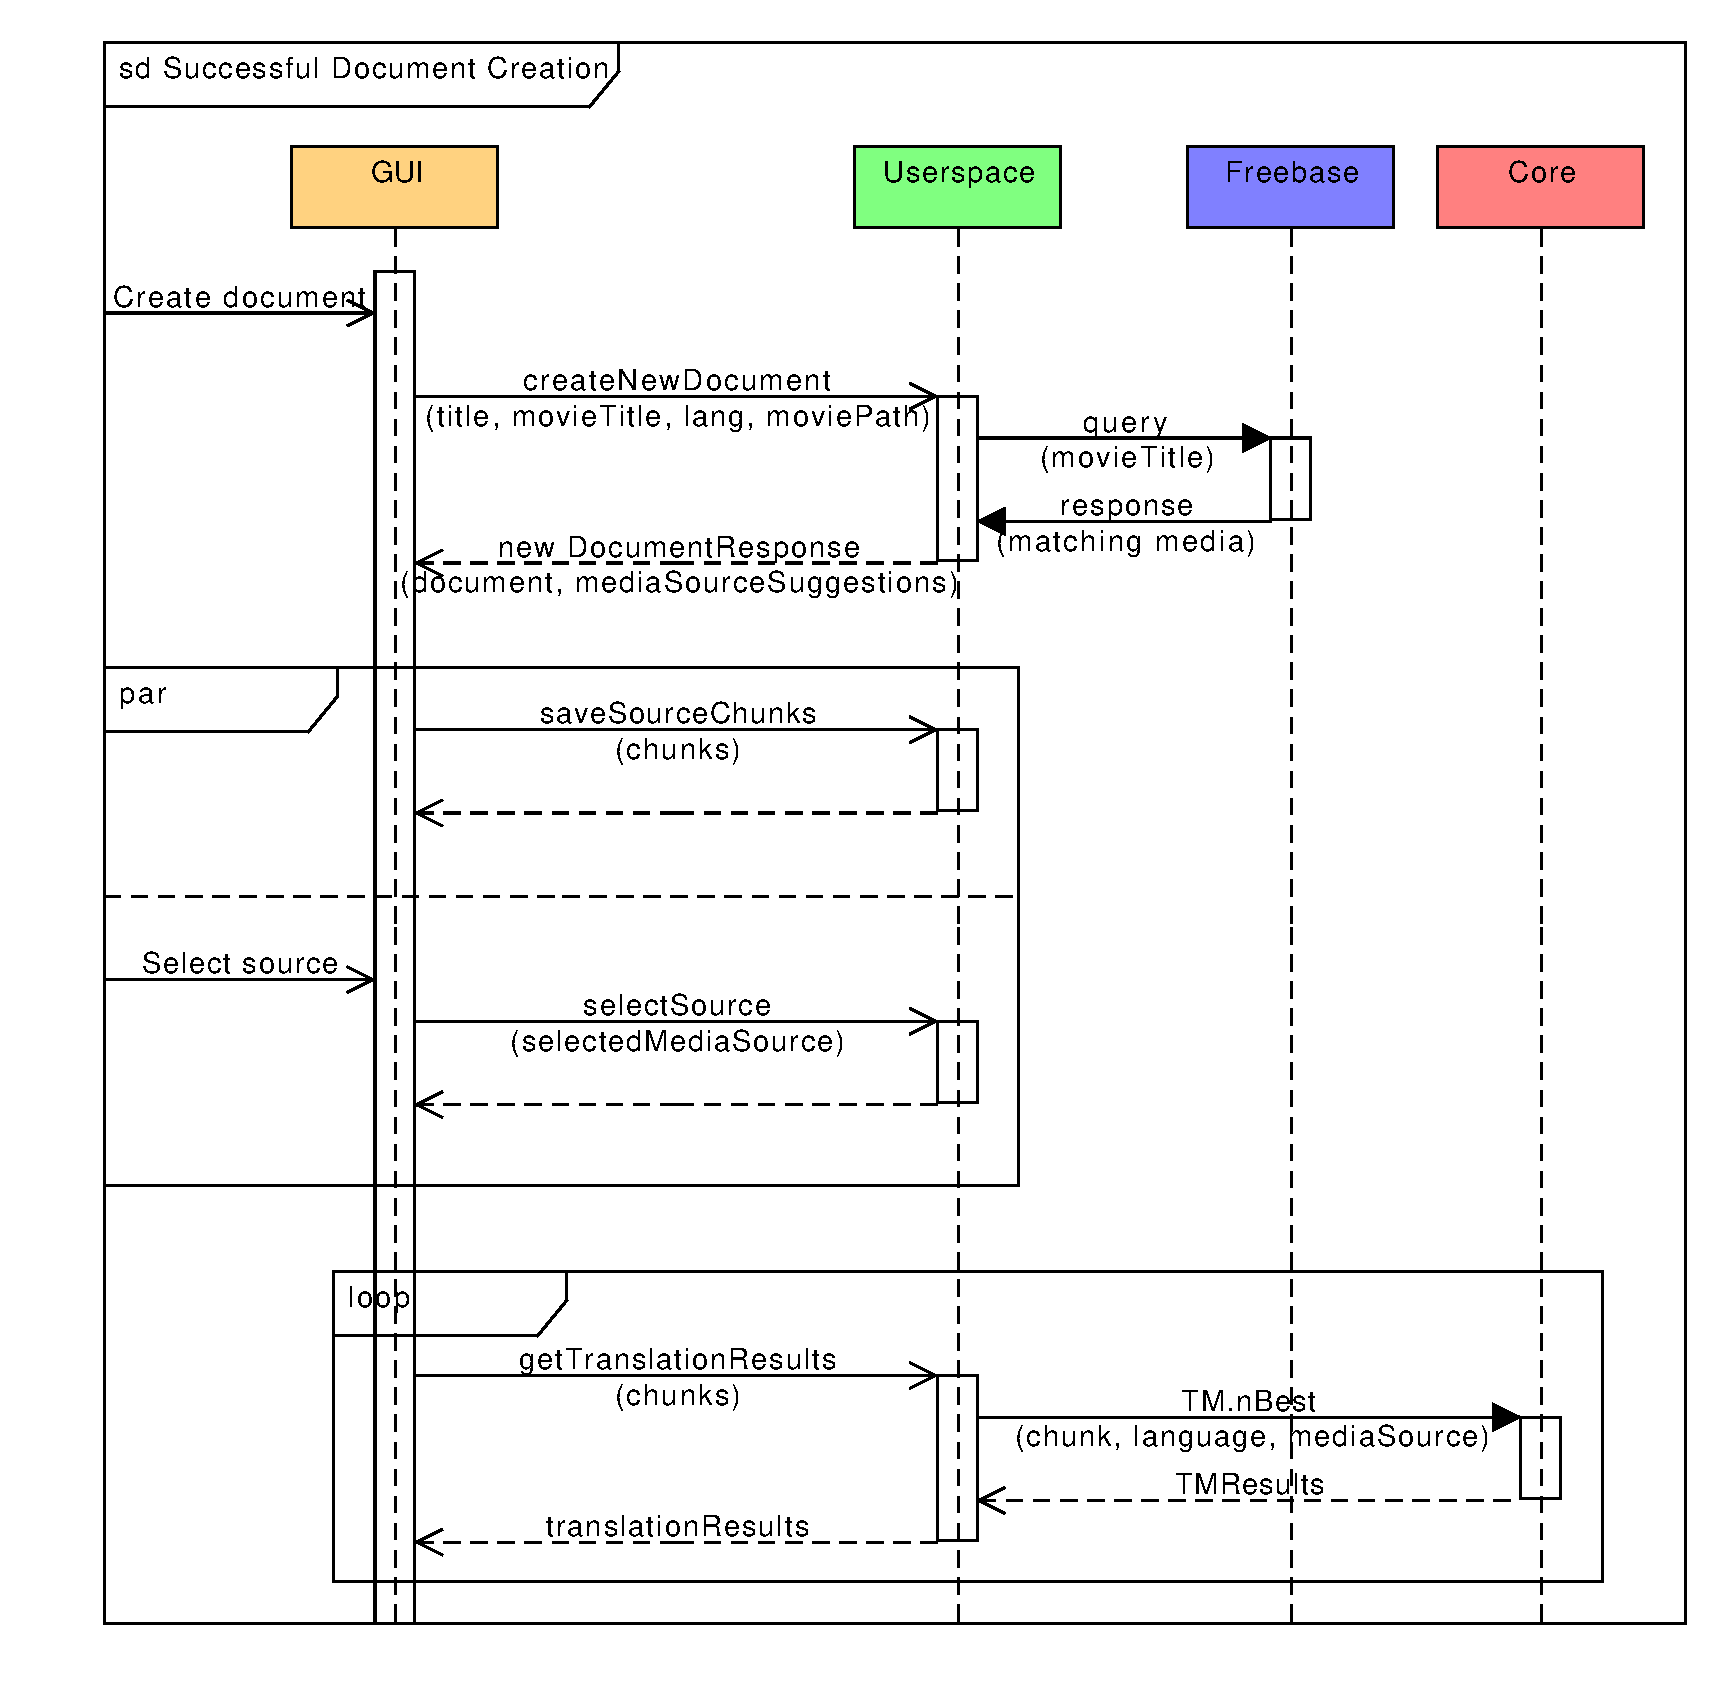
\includegraphics[scale=0.65]{figures/document_creation_sequence_RPC.pdf}
\end{center}
\caption{Sequence diagram of document creation, including translation suggestions loading.}\label{rpc:sd:document_creation}
\end{figure}

\section{User Registration and Login}
\label{sec:rpc:login}

The user is required to log in to use the application.

The users are logged in if they have a valid {\tt sessionID} which is linked to their user accounts.
The {\tt sessionID} expires after a given period of time without any user interaction with the server (1 hour by default).

Two ways to log in are supported -- Simple Login and OpenID Login; these are further described separately. The only two common methods are {\tt checkSessionID} and {\tt logout}, which are therefore described first.

\subsubsection{SessionResponse checkSessionID(String sessionID)}
Validates the given {\tt sessionID}. To be used with a {\tt sessionID} that does not result from invoking neither {\tt simpleLogin} nor {\tt getSessionID} (such as a {\tt sessionID} stored in a cookie).
Returns a {\tt SessionResponse} instance containing the {\tt sessionID} and the {\tt User} object if the {\tt sessionID} is valid, or null otherwise.

\subsubsection{Void logout(String sessionID)}
Invalidate the user session with the given {\tt sessionID}.

\subsection{Simple Login and Registration}
\label{subsec:simple_login}

The Simple Login is the classical implementation of user login. Each user must first register with a unique username and a password of choice. These credentials are then used to log into the application. (The password is to be stored on the server side in the form of a one-way hash.)

The users can also provide an e-mail address for forgotten password retrieval. They then has the option to request a password reset e-mail, based on his username or the e-mail address. The password reset e-mail contains a link to a page where the user can set a new password, based on a temporary password change token.

\subsubsection{Boolean registration(String username, String password, String email)}
Register a user with the given username and password, also setting the e-mail address if provided and sending registration info to it.
Returns true on success, false if the username is already taken, and an exception in case of other errors (usually an invalid e-mail address).

\subsubsection{SessionResponse simpleLogin(String username, String password)}
Try to log in the user with the given username and password.
Returns a {\tt SessionResponse} instance containing the {\tt sessionID} and the User object on success, or null if the credentials are invalid.

\subsubsection{Boolean sendChangePasswordMail(String username)}
Send a password reset e-mail
to the e-mail address of the user with the given username.
Returns true if the e-mail is successfully sent;
returns false if the username is not registered or there is no e-mail address stored with the corresponding user account.

\subsubsection{Boolean sendChangePasswordMailByMail(String email)}
Send a password reset e-mail to the given e-mail address.
The password reset link is bound to a username;
therefore, if there are multiple user accounts with the given e-mail address,
multiple password reset e-mail are sent to the e-mail address.
Returns true if the e-mail is successfully sent;
returns false if the e-mail address is not registered with any user account.

\subsubsection{Boolean changePassword(String username, String password, String token)}
\label{sec:rpc_changePassword}
Set a new password in case of forgotten password.
The temporary password change token must be still valid,
and identical to one sent in the password reset e-mail
to the user with the given username.
Returns true if the password change is successful;
returns false if the token is not valid.

\subsection{Login via OpenID Services}
\label{subsubsec:gui_openid}

This section describes the OpenID Login process. First, the three RPCs involved are introduced. Then, the whole process, also shown in the sequence diagram \ref{rpc:sd:openid_login}, is described.

\subsubsection{LoginSessionResponse getAuthenticationURL(AuthenticationServiceType serviceType)}
\label{sec:rpc_getAuthenticationURL}

Return the URL of a window to show to the user to log in using his OpenID account at an OpenID provider specified by {\tt serviceType}. It leads to a web page of the OpenID provider, with the return page set to the FilmTit application, to the {\tt AuthenticationValidationWindow} page.

A generated temporary one-time identifier, {\tt authID}, is also included in the response. It is used to pair the authentication process, which takes place in the newly opened window, with the main GUI window.

\subsubsection{Boolean validateAuthentication(int authID, String responseURL)}

Validate the response URL from the OpenID provider, which contains information about the result of the OpenID authentication.

If the authentication is found to have been successful, a new session is generated for the user and paired with the given {\tt authID}, and true is returned.
Otherwise, the method returns false.

\subsubsection{SessionResponse getSessionID(int authID)}

Check whether the user has already successfully logged in using his OpenID with the given {\tt authID}.

\begin{itemize}
\item If yes, the corresponding {\tt sessionID} and {\tt User} object are returned.
\item If not yet, but the {\tt authID} is valid, which means that an OpenID login operation is probably still in progress, null is returned.
\item Otherwise, an exception is thrown.
\end{itemize}

\subsubsection{The OpenID Login Process}
\label{subsubsec:gui:openid}

\begin{figure}[h]
\begin{center}
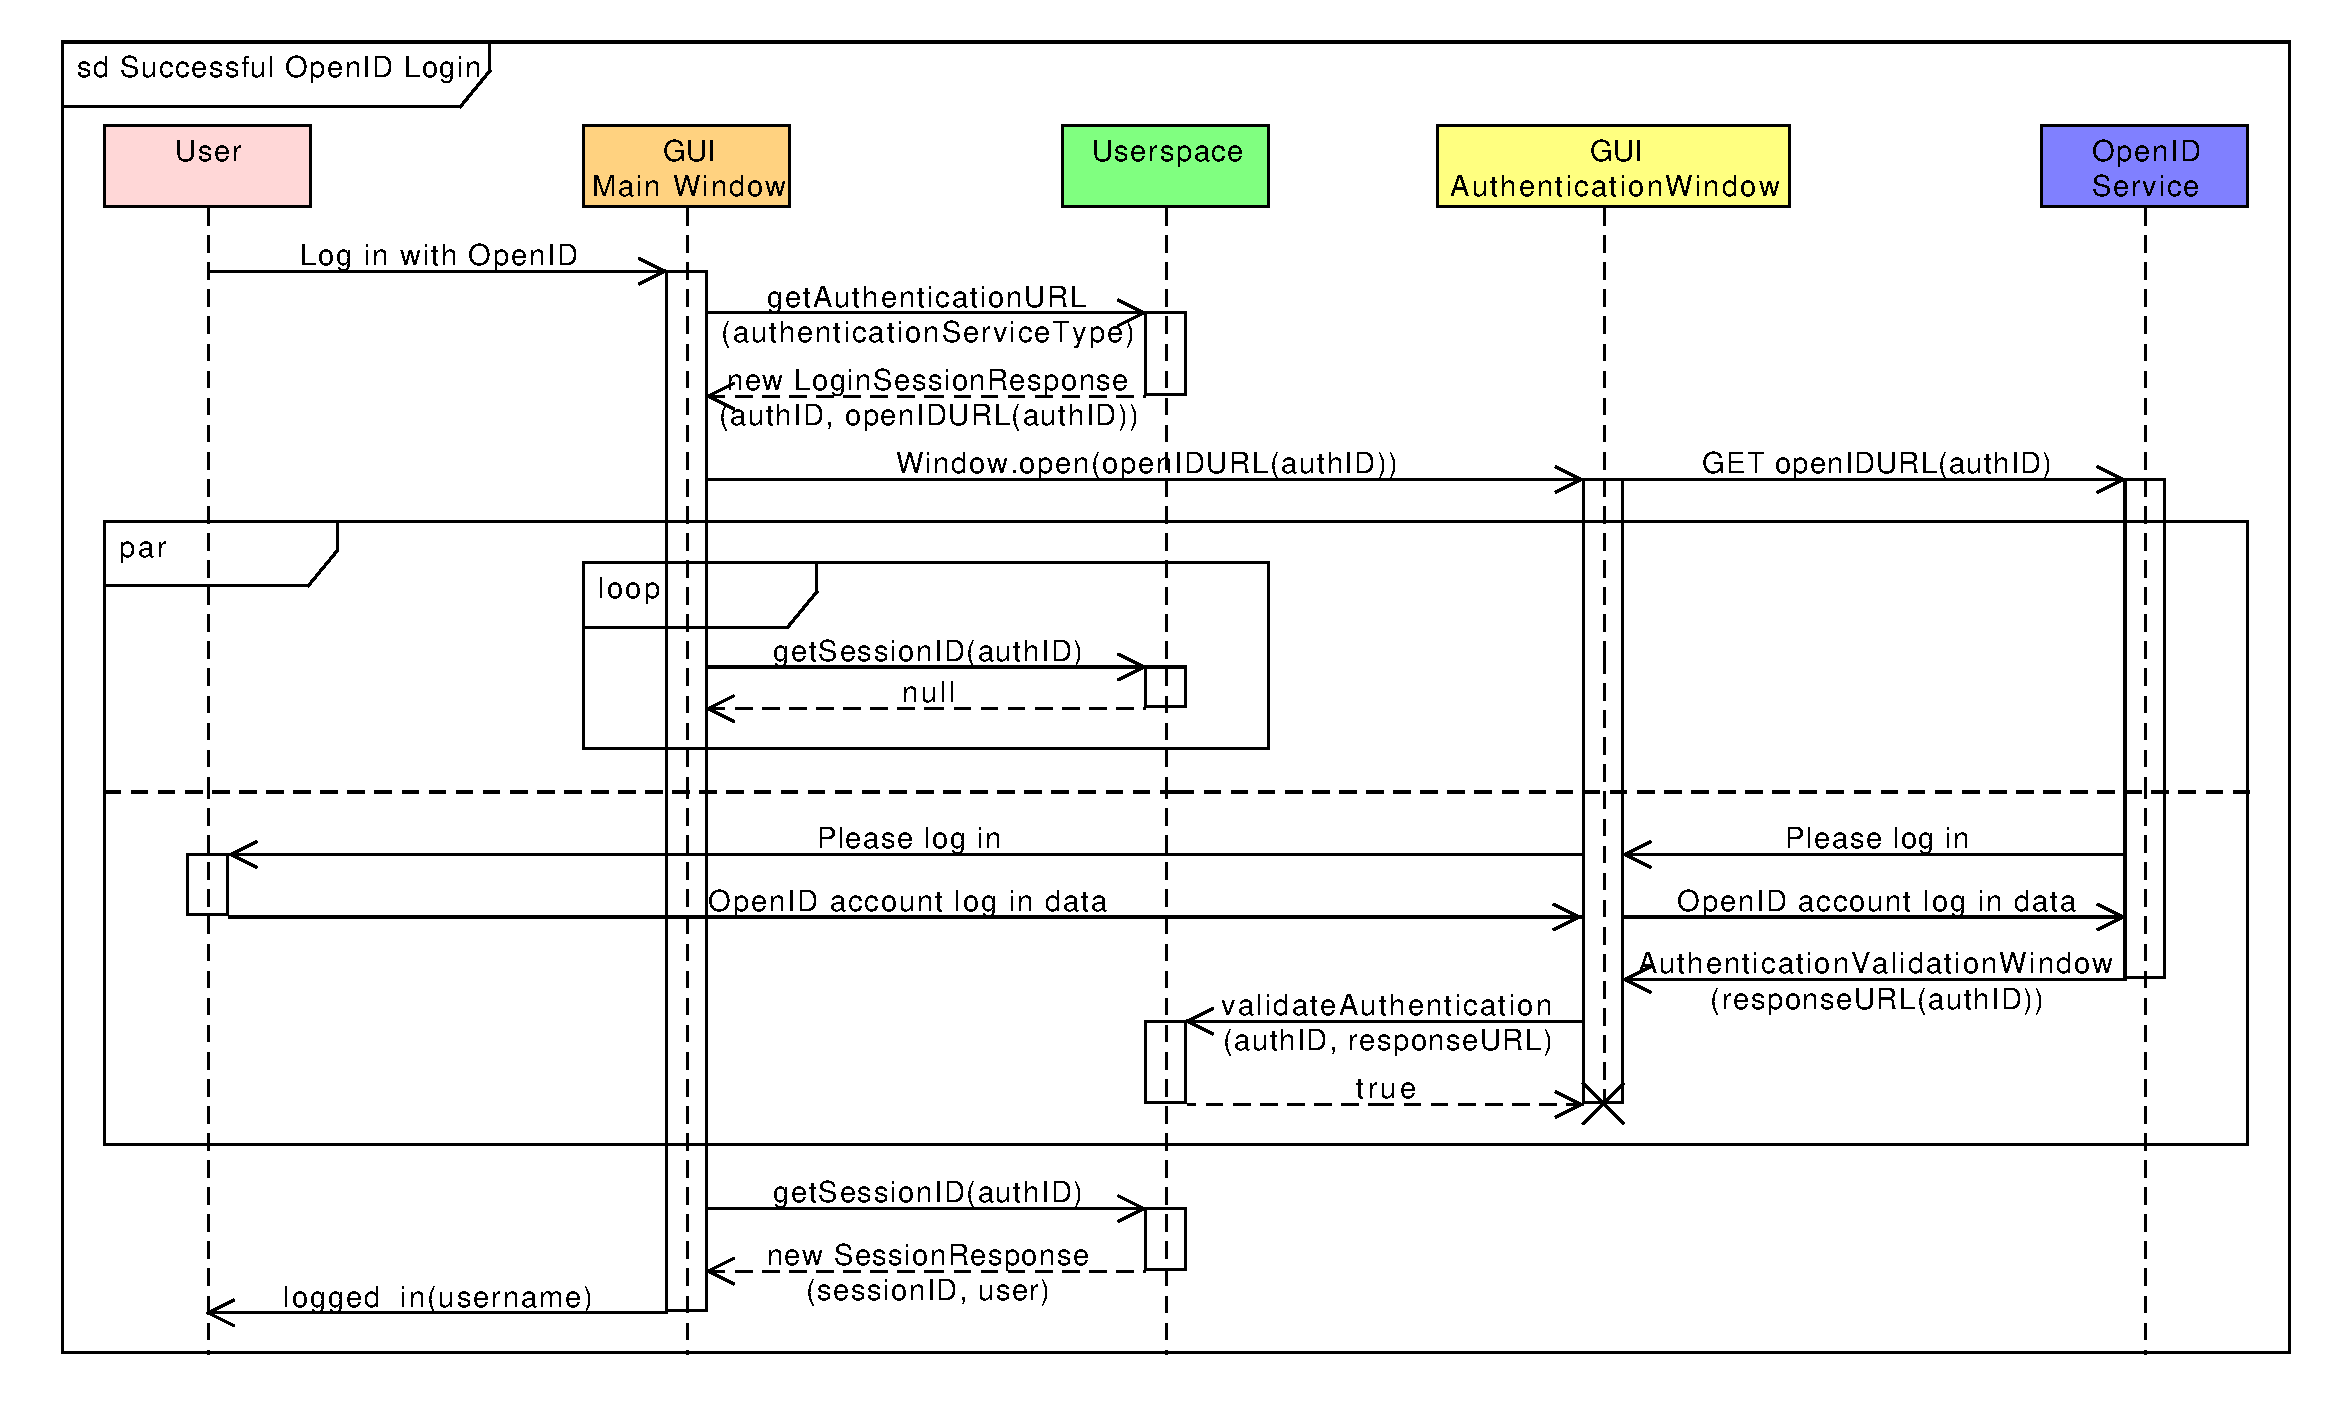
\includegraphics[scale=0.55, angle=90]{figures/openid_login_sequence.pdf}
\end{center}
\caption{Sequence diagram of OpenID login.}\label{rpc:sd:openid_login}
\end{figure}

The authentication itself is done in a new authentication window.
A successful authentication in the authentication window is then paired with the GUI main window using a temporary one-time identifier, {\tt authID}, shared by the User Space, the main GUI window and the authentication window.
(Because of JavaScript security restrictions, there is no simple way of sending the result of the authentication process from the authentication window to the main window;
however, the {\tt authID} can be sent to the new window easily because it is already known at the time of its creation.)

When OpenID Login is requested by the user, the GUI main window calls {\tt getAuthenticationURL} method.
The User Space generates an {\tt authID}, and a URL to be used for the authentication, and returns that to the GUI, which opens a new authentication window with the received URL.
The URL points to an OpenID provider web page (currently supported OpenID providers are Google, Yahoo and Seznam). As a GET parameter, it contains the return URL, which leads back to FilmTit -- to the {\tt AuthenticationValidationWindow} page, including the {\tt authID} as a GET parameter in the return URL.

After opening the authentication window, GUI starts waiting for the user to authenticate. The waiting is active, polling the User Space with {\tt getSessionID} in regular intervals until a non-null value is returned.

Meanwhile, the user can authenticate in the authentication window. The OpenID provider then redirects the user to the return URL, which is the {\tt AuthenticationValidationWindow}, together with parameters describing the result of the authentication and providing some information about the user.
The whole response URL is then sent through {\tt validateAuthentication} to User Space for validation.

If User Space finds the authentication to be successful, a new session is created for the user, and the {\tt sessionID} is stored in a pair with the {\tt authID}.
If a user with the given OpenID is not registered yet, registration is transparently performed at this moment; no explicit registration is required for OpenID login.
The authentication window is then closed.
In case of an error, the error message is displayed in the authentication window (and the window stays open).

When a successful authentication took place, the {\tt getSessionID} method returns the {\tt sessionID} and a {\tt User} object, the polling stops and the authentication process is completed.

\section{User Settings}
\label{sec:rpc:settings}

There are several settings that the user can change. There is a separate call for each of the settings -- therefore, a set of individual calls must be invoked if the user decides to change multiple settings at once, and each of the calls can succeed or fail independently on the results of the other calls.

The settings are stored in the {\tt User} object and sent to GUI on login, as a part of the {\tt SessionResponse} which is the result of the methods {\tt simpleLogin}, {\tt getSessionID} and {\tt checkSessionID}. There is no dedicated method to load the settings; {\tt checkSessionID} is to be used for that purpose.

\subsection{Account and Logging in Settings}

\subsubsection{Void setUsername(String sessionID, String username)}
Change user's username.

\subsubsection{Void setPassword(String sessionID, String password)}
Change user's password.

\subsubsection{Void setEmail(String sessionID, String email)}
Change user's e-mail.

\subsubsection{Void setPermanentlyLoggedIn(String sessionID, boolean permanentlyLoggedIn)}
Stay logged in permanently (for 1 month) instead of 1 hour (sets the session timeout). The time out times configurable, for details see \ref{subsec:user_scpace_settings}.

\subsection{Translation Workspace Settings}

\subsubsection{Void setMaximumNumberOfSuggestions(String sessionID, int number)}
Set maximum number of suggestions to show for each line.

\subsubsection{Void setUseMoses(String sessionID, boolean useMoses)}
Include Machine Translation results in translation suggestions.

\section{Remote Logging}
\label{sec:rpc:remotelog}

The remote logging is used to log messages from GUI on server. The messages are to be printed in the server log and can also be stored in the database.

\subsubsection{Void logGuiMessage(LevelLogEnum level, String context, String message, String sessionID)}
Log the given message from GUI on server.
The supported levels are \emph{DebugNotice}, \emph{Notice}, \emph{Warning} and \emph{Error}.
The context specifies the type of the message and should be constant for each instance of a similar message; it can contain e.g.\ a class name, a method name or an RPC name. The message should be as detailed as to provide all necessary information, including e.g.\ values of variables or a stack trace if applicable.

The {\tt sessionID} is only used to include the {\tt userID} in the logged message; it is to be null if the user is not logged in.

\section{Exceptions Thrown by RPCs}
\label{sec:rpc:exceptions}

The RPCs typically throw an exception on failure. These exceptions should be of only four types, described in this section.

\subsection{InvalidSessionIdException}

Most of the RPCs can only be invoked by a logged in user -- such RPCs take the {\tt sessionID} as their first parameter and throw an {\tt InvalidSessionIdException} in case of an invalid {\tt sessionID}. Typically the ID would be originally valid but expired, so the expected reaction to this exception is to simply ask the user to log in again.

\subsection{InvalidDocumentIdException}

RPCs that manipulate the document usually take the {\tt documentID} as a parameter and throw an {\tt InvalidDocumentIdException} if a document with the given ID does not exist or does not belong to the user.

\subsection{InvalidChunkIdException}

RPCs that manipulate individual chunks take either the whole chunks or only their indexes as a parameter. They throw an {\tt InvalidChunkIdException} if the specified chunk does not exist.

\subsection{InvalidValueException}

The {\tt InvalidValueException} is thrown by a method if a value provided by the user, such as an e-mail address or a password, does not have the required format. It always contains details about the nature of the error as the message, which usually should be shown to the user.
